\documentclass[aspectratio=169,11pt]{beamer}

% Shared style (ib-tutorials.sty at the repo root).
\makeatletter\def\input@path{{./}{../}}\makeatother
\usepackage{ib-tutorials}

\usepackage[utf8]{inputenc}
\usepackage{amsmath,amssymb}
\usepackage{booktabs}
\usepackage{array}
\usepackage{graphicx}
\usepackage{xcolor}
\usepackage{listings}
\usepackage{tikz}
\usetikzlibrary{arrows.meta,positioning,shapes.geometric,fit,calc}
\usepackage{hyperref}

\newcommand{\sourcecredit}[1]{\vfill\begin{flushright}\tiny\textcolor{DarkGray}{#1}\end{flushright}}
\newcolumntype{L}[1]{>{\raggedright\arraybackslash}p{#1}}

% Part X: every slide carries the legacy label.
\setbeamertemplate{background}{\begin{tikzpicture}[remember picture,overlay]
  \node[anchor=north east,font=\tiny\sffamily,text=DarkGray,fill=LightGray!50,rounded corners=1pt,inner sep=2pt]
    at ([xshift=-2mm,yshift=-1.2mm]current page.north east) {LEGACY \textbullet\ Part X, archive};
\end{tikzpicture}}

\lstset{
  basicstyle=\ttfamily\scriptsize\color{BlackGray},
  keywordstyle=\color{NavyBlue}\bfseries,
  commentstyle=\color{DarkGray}\itshape,
  stringstyle=\color{OliveGreen},
  showstringspaces=false,
  columns=fullflexible,
  keepspaces=true,
  frame=single,
  framerule=0.4pt,
  rulecolor=\color{LightGray},
  backgroundcolor=\color{LightGray!30},
  xleftmargin=0.25em,
  xrightmargin=0.25em,
  breaklines=true,
  breakatwhitespace=true
}
\lstdefinestyle{shell}{morecomment=[l]{\#}}
\lstdefinestyle{cpp}{language=C++,morekeywords={nullptr}}
\lstdefinestyle{cpptiny}{language=C++,morekeywords={nullptr},basicstyle=\ttfamily\tiny\color{BlackGray}}
\lstdefinestyle{make}{morecomment=[l]{\#}}
\lstdefinestyle{maketiny}{morecomment=[l]{\#},basicstyle=\ttfamily\tiny\color{BlackGray}}
\lstdefinestyle{plaintiny}{basicstyle=\ttfamily\tiny\color{BlackGray}}

\title[X3 Old code, mapped to current code]{X3. Old IBAMR and libMesh code, mapped to current code}
\subtitle{How to read the course and lab programs of 2009--2024, what each old pattern was, and what it is in IBAMR 0.16 and 0.19 with CMake: a map for porting, labelled legacy}
\author[Miller]{Laura A. Miller}
\institute[UArizona]{Department of Mathematics, University of Arizona}
\date{Using IB Software \textbullet\ Part X, archive \textbullet\ Chapter X3}


\begin{document}

% 1
\begin{frame}[plain]
\maketutorialtitlepanel{%
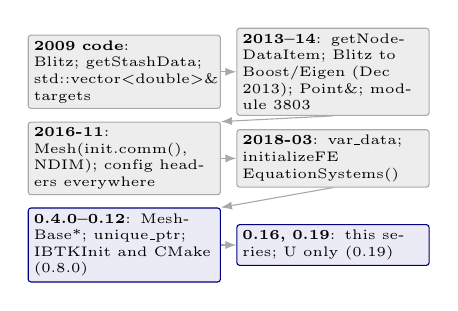
\begin{tikzpicture}[every node/.style={font=\tiny}, era/.style={draw=DarkGray, fill=LightGray!40, rounded corners=1pt, align=left, inner sep=2pt, text width=2.3cm}]
  \node[era] (a) at (0,0) {\textbf{2009 code}: Blitz; \code{getStashData}; \code{std::vector<double>\&} targets};
  \node[era] (b) at (2.65,0) {\textbf{2013--14}: \code{getNodeDataItem}; Blitz to Boost/Eigen (Dec 2013); \code{Point\&}; module 3803};
  \node[era] (c) at (0,-1.1) {\textbf{2016-11}: \code{Mesh(init.comm(), NDIM)}; config headers everywhere};
  \node[era] (d) at (2.65,-1.1) {\textbf{2018-03}: \code{var\_data}; \code{initializeFE\allowbreak EquationSystems()}};
  \node[era,draw=NavyBlue,fill=NavyBlue!8] (e) at (0,-2.2) {\textbf{0.4.0--0.12}: \code{MeshBase*}; \code{unique\_ptr}; \code{IBTKInit} and CMake (0.8.0)};
  \node[era,draw=NavyBlue,fill=NavyBlue!8] (f) at (2.65,-2.2) {\textbf{0.16, 0.19}: this series; \code{U} only (0.19)};
  \draw[-{Latex[length=1.4mm]},DarkGray] (a) -- (b); \draw[-{Latex[length=1.4mm]},DarkGray] (b.south) -- (c.north east);
  \draw[-{Latex[length=1.4mm]},DarkGray] (c) -- (d); \draw[-{Latex[length=1.4mm]},DarkGray] (d.south) -- (e.north east);
  \draw[-{Latex[length=1.4mm]},DarkGray] (e) -- (f);
\end{tikzpicture}}
\end{frame}

% 2
\begin{frame}{How to use this chapter}
\label{fr:use}
\begin{columns}[T,onlytextwidth]
\begin{column}{0.52\textwidth}
\small
\begin{itemize}\setlength{\itemsep}{3pt}
  \item \al{Legacy.} Every code line marked ``old'' here is history, quoted with its era and file so that you can recognize it. Do not type it: the ``new'' line, from this series' examples or from IBAMR 0.19.0's headers, is what to write.
  \item \al{First date the code} (slides \ref{fr:dating}--\ref{fr:dating2}): the Makefile's paths tell you which IBAMR it was written for.
  \item \al{Then follow the map}: one slide per kind of change, in the order a port meets them (build, compile, run, look at the output); slides \ref{fr:map1}--\ref{fr:map3} map every folder of \code{examples/legacy}, and four 2013--14 examples, to its maintained example (or to none).
\end{itemize}
\end{column}
\begin{column}{0.45\textwidth}
\begin{punchbox}
\small The short version is chapter 3's porting checklist; this chapter is its long form, with the history of each change. ``Changed in'' gives an IBAMR version only where IBAMR's changelog states it; otherwise the bracket between two course installs.
\end{punchbox}
\vspace{2mm}
\footnotesize The code quoted comes from the 2014 and 2016-11 course folders and those kept in \code{examples/legacy}, the 2014 lab examples, the course decks and install notes (2012--2024) and IBAMR 0.19.0's source.
\end{column}
\end{columns}
\end{frame}

% 3
\begin{frame}{Dating old code by its Makefile path (1/2): UNC, 2011--2020}
\label{fr:dating}
\small Open the Makefile and read the two lines that point at IBAMR: \code{IBAMR\_SRC\_DIR}, the source, and \code{IBAMR\_BUILD\_DIR}, the compiled library. Their paths say where and when the program was built.

\vspace{2mm}
\scriptsize
\renewcommand{\arraystretch}{1.1}
\setlength{\tabcolsep}{4pt}
\begin{tabular}{@{}L{0.44\textwidth}L{0.53\textwidth}@{}}
\toprule
path in the Makefile & what it means \\
\midrule
\code{\$(HOME)/sfw2/...} & a source build in a home folder on UNC's KillDevil, 2012--13 (chapter X2) \\
\code{/usr/bin/sfw/...} & the lab's own Linux machine, built as root, 2011--13 (chapter X2) \\
\code{/nas02/apps/ibamr-3803/OFED-1.5.2/IBAMR2} & UNC's module \code{ibamr/3803} (Kure and KillDevil, about February 2014): probably SVN revision 3803, older than IBAMR's first tag, v0.1-rc1 (May 2014) \\
\code{/nas02/apps/ibamr-2016-11/...} & UNC's module \code{ibamr/2016-11} (November 2016): the course's 2016--17 ports \\
\code{/nas/longleaf/apps-dogwood/\allowbreak ibamr/2018-03/...} & UNC's Dogwood, module \code{ibamr/2018-03} (March 2018): a snapshot of IBAMR from before 0.3.0; most UNC folders of \code{examples/legacy} \\
\code{/nas/longleaf/apps-dogwood/\allowbreak ibamr/0.6.0/...} & Dogwood's module \code{ibamr/0.6.0} (2020): the UNC folders \code{7-*} and \code{9-*} \\
\bottomrule
\end{tabular}
\sourcecredit{The Makefiles of \code{examples/legacy} and of the 2014 and 2016-11 course folders; IBAMR's release tags; the instructor's install notes; the code check of October 2026.}
\end{frame}

% 3b
\begin{frame}[fragile]{Dating old code by its Makefile path (2/2): Arizona, and this series}
\label{fr:dating2}
\scriptsize
\renewcommand{\arraystretch}{1.1}
\setlength{\tabcolsep}{4pt}
\begin{tabular}{@{}L{0.44\textwidth}L{0.53\textwidth}@{}}
\toprule
path in the Makefile & what it means \\
\midrule
\code{/contrib/<group>/ibamr/0.7.1/...} & a University of Arizona build of IBAMR 0.7.1 (the UA rubber band; the AZ copies of the rubber band, moving cylinders and triangle in \code{originals/Old files}) \\
\code{/groups/<group>/ib10/...} & the UA autotools build of 2022--24, used by almost all UA folders; 0.10 judged from the folder name only \\
\code{/groups/<group>/ib16/...} & a UA autotools build of July 2025, presumably 0.16 \\
no Makefile, a \code{CMakeLists.txt} with \code{find\_package(IBAMR 0.16.0)} & this series' examples: IBAMR 0.16.0 and 0.19.0, built by autoibamr (chapter 2) \\
\bottomrule
\end{tabular}

\vspace{2mm}
\footnotesize The UA rubber band's Makefile, for example:
\begin{lstlisting}[style=maketiny]
IBAMR_SRC_DIR = /contrib/<group>/ibamr/0.7.1/include/IBAMR
IBAMR_BUILD_DIR = /contrib/<group>/ibamr/IBAMR-0.7.1
LIBSNEW = $(LIBS) -lnetcdf -lcurl
\end{lstlisting}
An autotools Makefile includes \code{\$(IBAMR\_BUILD\_DIR)/config/make.inc} near its top; autoibamr installs no \code{make.inc}, and the next release, IBAMR 0.20 (in development in October 2026), removes autotools altogether. A Makefile path is therefore a date, not a recipe: today's examples build with CMake (slide \ref{fr:build}).
\sourcecredit{\code{examples/legacy/UA-Examples} Makefiles and \code{originals/IBAMR Lectures/Files/Makefile} (\code{<group>} in place of the group's name); IBAMR's release tags; the code check of October 2026.}
\end{frame}

% 4
\begin{frame}{Five eras of one example: the rubber band}
\label{fr:eras}
\scriptsize
\renewcommand{\arraystretch}{1.05}
\begin{tabular}{@{}L{0.17\textwidth}L{0.77\textwidth}@{}}
\toprule
era & what the step changed in \code{main} \\
\midrule
2014 (module 3803) & \code{PetscInitialize(\&argc,\&argv,PETSC\_NULL,PETSC\_NULL)}; the \code{*\_prefix\_config.h} includes commented out; \code{app\_namespaces.h} in the middle of the includes; \code{.isNull()} tests \\
2016-11 & \code{IBAMR\_config.h}, \code{IBTK\_config.h}, \code{LData.h} and \code{LDataManager.h} added (November 2016; the other 2016-11 mains mark them ``added for MODULE 2016-11 NAB'', N. Battista, and the headers ``Added for IBAMR KD Module 2016-11 by NAB (1/27/17)''); \code{app\_namespaces.h} moved after all other includes \\
2018-03 (Dogwood) & a fresh copy of IBAMR's \code{IB/explicit/ex1} main, adapted: \code{NULL}, a solver-type switch, named \code{Pointer<CartGridFunction>} objects, the \code{periodic\_shift} loop \\
UA, 0.7.1 and \code{ib10} (2020--24) & the same main; an input whose lines end with \code{//} again, as in 2014 (a Windows line-ending workaround, slide \ref{fr:inputs2}) \\
0.16 / 0.19 & \code{IBTKInit}; config headers gone; \code{IBTK::rel\_equal\_eps}, \code{IBTK\_MPI}; \code{nullptr}; \code{snprintf}; \code{PetscInt}; a \code{CMakeLists.txt} \\
\bottomrule
\end{tabular}

\vspace{1mm}
\footnotesize ``I was only able to get a working IB example by taking more recent main, makefile, and input files and modifying them for my example'' (the 2018 Dogwood porting slides): that is why the 2018 mains look like upstream's, and why the next slides follow the order of a port rather than the history.
\sourcecredit{Era-to-era diffs of the rubber band's \code{main} (2014, 2016-11, 2018-03, UA, IB/01); the instructor's 2018 porting slides.}
\end{frame}

% 5
\begin{frame}[fragile]{Build: a Makefile with \code{make.inc}, then CMake}
\label{fr:build}
\begin{columns}[T,onlytextwidth]
\begin{column}{0.49\textwidth}
\textbf{Old} (the rubber band's Makefile, 2014)
\begin{lstlisting}[style=maketiny]
IBAMR_SRC_DIR = /nas02/apps/ibamr-3803/OFED-1.5.2/IBAMR2
IBAMR_BUILD_DIR = /nas02/apps/ibamr-3803/ibamr-objs-opt
...
include $(IBAMR_BUILD_DIR)/config/make.inc
...
SOURCES = main.C update_target_point_positions.C ...
OBJS = main.o update_target_point_positions.o update_springs.o
main2d:
	if (test -f stamp-3d); then $(MAKE) clean; fi
	touch stamp-2d
	$(MAKE) PDIM=2 main-2d
\end{lstlisting}
\end{column}
\begin{column}{0.49\textwidth}
\textbf{New} (IB/01's \code{CMakeLists.txt})
\begin{lstlisting}[style=maketiny]
cmake_minimum_required(VERSION 3.15...3.30)
project(ib01_rubber_band LANGUAGES C CXX)
find_package(IBAMR 0.16.0 REQUIRED)
add_executable(main2d main.cpp)
target_link_libraries(main2d PRIVATE IBAMR::IBAMR2d)
\end{lstlisting}
\begin{lstlisting}[style=shell,basicstyle=\ttfamily\tiny\color{BlackGray}]
cmake -S . -B build -DCMAKE_BUILD_TYPE=Release
cmake --build build -j 4
mpirun -np 4 ./build/main2d input2d
\end{lstlisting}
\footnotesize Extra sources go into \code{add\_executable}; 3D uses \code{IBAMR::IBAMR3d} and \code{main3d}.
\end{column}
\end{columns}
\vspace{1mm}
\footnotesize \al{Today's error} with an old Makefile: \code{Makefile:27: /contrib/<group>/ibamr/IBAMR-0.7.1/config/make.inc: No such file or directory} (chapter 3). \al{Changed in} 0.8.0: ``IBAMR can now be configured, compiled, and installed with CMake instead of with autotools''.
\sourcecredit{The 2014 course Makefile; \code{examples/IB/01-rubber-band}; IBAMR's changelog 0.7.1 to 0.8.0; chapter 3.}
\end{frame}

% 6
\begin{frame}{Makefile leftovers: \code{LIBSNEW}, \code{-lnetcdf -lcurl}, stamps, \code{.C} files}
\label{fr:leftovers}
\small
\begin{itemize}\setlength{\itemsep}{3pt}
  \item \al{\code{LIBSNEW}.} The 2014 IBFE decks said ``At the beginning of the Makefile declare LIBSNEW'', \code{LIBSNEW = \$(LIBS) -lnetcdf -lcurl}, ``Use this instead of the \$(LIBS) flag''. The 2014 IBFE Makefiles link with \code{\$(LIBSNEW)}, and so do five UNC and two UA IBFE Makefiles of 2018--24. Sixteen of the 21 UNC Makefiles write \code{LIBS = \$(LIBS) -lnetcdf -lcurl} instead: a dead line, since the \code{make.inc} included after it sets \code{LIBS} again. Neither is needed today: netCDF has come in through libMesh since IBAMR 0.6.0, and a CMake build has no such line.
  \item \al{Stamps.} \code{stamp-2d} and \code{stamp-3d} made \code{make} clean the objects when you switched dimension; with CMake, \code{main2d} and \code{main3d} are separate targets.
  \item \al{File names.} \code{main.C} and \code{update\_*.C} became \code{main.cpp} and \code{update\_*.cpp} in this series (CMake accepts \code{.C}); IBAMR's own examples are \code{example.cpp}.
  \item \al{One program instead of near-copies}: IBFE/01 (\code{MOTION}) and IBFE/06 (\code{FIBER\_MODE}) replace three course folders each with one input key.
\end{itemize}
\sourcecredit{The 2014 IBFE Makefile slides; \code{examples/legacy} Makefiles; the October 2026 code check (C1); the maintained READMEs.}
\end{frame}

% 7
\begin{frame}[fragile]{Configuration headers through four eras}
\label{fr:config}
\begin{columns}[T,onlytextwidth]
\begin{column}{0.5\textwidth}
\footnotesize
\begin{itemize}\setlength{\itemsep}{2pt}
  \item \al{Up to 2013}: \code{\#include <IBAMR\_prefix\_config.h>}, \code{<IBTK\_prefix\_config.h>}. The December 2013 notes and the 2014 module slides say to comment them out; the 2014 code has them commented.
  \item \al{2014 IBFE and 2016--2024}: \code{IBAMR\_config.h}, \code{IBTK\_config.h}, \code{SAMRAI\_config.h}, added to every IB program and every \code{update\_*.h} for module 2016-11.
  \item \al{Now}: delete the first two and keep \code{<SAMRAI\_config.h>}; \code{ibamr/app\_namespaces.h} already includes \code{<ibamr/config.h>}.
\end{itemize}
\end{column}
\begin{column}{0.48\textwidth}
\begin{lstlisting}[style=cpptiny]
// 2016-11, update_beams.h
#include <IBAMR_config.h>    //Added for IBAMR KD Module 2016-11 by NAB (1/27/17)
#include <IBTK_config.h>
#include <SAMRAI_config.h>
\end{lstlisting}
\footnotesize In IBAMR's autotools templates today: \code{\#pragma message("This file has been deprecated: use ibamr/config.h instead")}.
\end{column}
\end{columns}
\vspace{1mm}
\footnotesize \al{Today's error} (almost every course program stops here first; the three UA fiber-stress programs and the 2014 IB programs do not include \code{IBAMR\_config.h} or \code{IBTK\_config.h}): \code{main.cpp:31:10: fatal error: IBAMR\_config.h: No such file or directory}. CMake installs have no \code{IBAMR\_config.h} or \code{IBTK\_config.h}; the version of the deprecation is not stated.
\sourcecredit{The instructor's December 2013 and March 2014 notes; the 2016-11 course code; IBAMR 0.19.0's \code{config/IBAMR\_config.h.tmp.in}; chapter 3.}
\end{frame}

% 8
\begin{frame}[fragile]{Includes that belong where}
\label{fr:includes}
\begin{columns}[T,onlytextwidth]
\begin{column}{0.5\textwidth}
\footnotesize
\begin{itemize}\setlength{\itemsep}{2pt}
  \item 2014: \code{<ibamr/app\_namespaces.h>} in the middle of \code{main}'s includes, and inside \code{update\_*.h} headers.
  \item 2016-11: \code{\#include <ibtk/LData.h> //added for MODULE 2016-11 NAB} before \code{<ibtk/LDataManager.h>}; \code{app\_namespaces.h} moved after all other includes; each \code{update\_*.h} got about twenty includes.
  \item The lab's 2013 notes had already added \code{\#include <ibtk/LDataManager.h>} to \code{main.C} on the lab's machine.
  \item IBTK's rule, in \code{app\_namespaces.h}: ``This header file may be included in application codes, but it MUST NOT be included in any other header (.h) or inline (-inl.h) file in the library.''
\end{itemize}
\end{column}
\begin{column}{0.48\textwidth}
\textbf{New} (IB/07's \code{update\_target\_point\_positions.h})
\begin{lstlisting}[style=cpptiny]
#include <ibtk/LData.h>
#include <ibtk/LDataManager.h>
#include <PatchHierarchy.h>
...
void update_target_point_positions(
    SAMRAI::tbox::Pointer<SAMRAI::hier::PatchHierarchy<NDIM> > hierarchy,
    IBTK::LDataManager* l_data_manager, ...);
\end{lstlisting}
\footnotesize Fully qualified types, no \code{app\_namespaces.h}. ``IBAMR 0.16 needs LData.h for LDataManager.h to compile; 0.19 does not.''
\end{column}
\end{columns}
\sourcecredit{The 2014 and 2016-11 course code; the 2017 deck ``How to update examples to new install''; \code{examples/IB/07-moving-plates}; IBAMR 0.19.0.}
\end{frame}

% 9
\begin{frame}[fragile]{Starting IBAMR: \code{PetscInitialize} and SAMRAI, then \code{IBTKInit}}
\label{fr:ibtkinit}
\begin{columns}[T,onlytextwidth]
\begin{column}{0.49\textwidth}
\textbf{Old} (IB, 2018--2024; 2014 and 2016-11 with \code{PETSC\_NULL})
\begin{lstlisting}[style=cpptiny]
PetscInitialize(&argc, &argv, NULL, NULL);
SAMRAI_MPI::setCommunicator(PETSC_COMM_WORLD);
SAMRAI_MPI::setCallAbortInSerialInsteadOfExit();
SAMRAIManager::startup();
...
SAMRAIManager::shutdown();
PetscFinalize();
\end{lstlisting}
IBFE: \code{LibMeshInit init(argc, argv);} instead of \code{PetscInitialize}.
\end{column}
\begin{column}{0.49\textwidth}
\textbf{New} (IB/01; IBFE/01 adds the second line)
\begin{lstlisting}[style=cpptiny]
IBTKInit ibtk_init(argc, argv, MPI_COMM_WORLD);
const LibMeshInit& init = ibtk_init.getLibMeshInit();
\end{lstlisting}
\footnotesize No shutdown calls: ``IBTKInit also shuts them down when it goes out of scope.''
\end{column}
\end{columns}
\vspace{1mm}
\footnotesize What \code{IBTKInit} does (0.19.0, \code{IBTKInit.cpp}): starts libMesh (or PETSc without it), calls \code{SAMRAIManager::setMaxNumberPatchDataEntries(2048)}, sets the SAMRAI and IBTK communicators, \code{setCallAbortInSerialInsteadOfExit}, \code{SAMRAIManager::startup()}; its destructor shuts down. \al{Changed in} 0.8.0: ``IBAMR now requires the initialization object IBTKInit to be created upon program start.'' The old start-up still compiles and runs (IBAMR's own \code{IB/explicit/ex0} and \code{IBFE/explicit/ex0} still use it), but keeps SAMRAI's default of 256 patch-data entries, a risk for runs with many variables (inferred, not observed).
\sourcecredit{\code{examples/legacy} mains; \code{examples/IB/01}, \code{IBFE/01}; IBAMR 0.19.0's \code{ibtk/src/utilities/IBTKInit.cpp} and changelog 0.7.1 to 0.8.0; chapter 3.}
\end{frame}

% 10
\begin{frame}[fragile]{\code{PETSC\_NULL}, \code{IBTK\_MPI} and the end-of-loop test}
\label{fr:mpi}
\begin{columns}[T,onlytextwidth]
\begin{column}{0.49\textwidth}
\textbf{Old}
\begin{lstlisting}[style=cpptiny]
PetscInitialize(&argc,&argv,PETSC_NULL,PETSC_NULL); // 2014, 2016-11
PetscInitialize(&argc, &argv, NULL, NULL);          // 2018-03
while (!MathUtilities<double>::equalEps(loop_time, loop_time_end)
       && time_integrator->stepsRemaining())
SAMRAI_MPI::sumReduction(&F_sum[0],NDIM);
\end{lstlisting}
\end{column}
\begin{column}{0.49\textwidth}
\textbf{New} (IB/01)
\begin{lstlisting}[style=cpptiny]
while (!IBTK::rel_equal_eps(loop_time, loop_time_end)
       && time_integrator->stepsRemaining())
IBTK_MPI::sumReduction(&F_sum[0], NDIM);
\end{lstlisting}
\end{column}
\end{columns}
\vspace{1mm}
\footnotesize
\begin{itemize}\setlength{\itemsep}{2pt}
  \item \code{PETSC\_NULL} became \code{NULL} between the course's 2016-11 and 2018-03 code; PETSc itself deprecated \code{PETSC\_NULL} in 3.19 (\code{PETSC\_DEPRECATED\_MACRO(3, 19, 0, "PETSC\_NULLPTR", )}), so old code compiles with a warning. With \code{IBTKInit} there is no \code{PetscInitialize} in user code at all.
  \item \al{Changed in} 0.8.0: ``All SAMRAI\_MPI calls in the library have been replaced with respective IBTK\_MPI calls.'' Optional in user code: \code{SAMRAI\_MPI::sumReduction} still exists, and \code{equalEps} still compiles.
\end{itemize}
\sourcecredit{The course mains of 2014, 2016-11 and 2018-03; \code{examples/IB/01}; PETSc 3.23.3's \code{petscsys.h}; IBAMR changelog 0.7.1 to 0.8.0.}
\end{frame}

% 11
\begin{frame}{Small things a fresh upstream \code{main} brings}
\label{fr:fresh}
\scriptsize
\renewcommand{\arraystretch}{1.05}
\begin{tabular}{@{}L{0.47\textwidth}L{0.47\textwidth}@{}}
\toprule
old (2014, 2016-11) & 2018-03 and now \\
\midrule
\code{... \&\& !app\_initializer->\allowbreak getVisItDataWriter().isNull();} & \code{... \&\& app\_initializer->\allowbreak getVisItDataWriter();} \\
\code{registerVelocityInitialConditions(new muParserCartGridFunction("u\_init", ...));} & a named \code{Pointer<CartGridFunction> u\_init = new muParserCartGridFunction(...);}, then \code{registerVelocityInitialConditions(u\_init);} \\
\code{new INSStaggeredHierarchyIntegrator(...)} & a \code{solver\_type} switch (\code{STAGGERED} or \code{COLLOCATED}) read from \code{Main} \\
\code{getPeriodicShift().min() > 0} and \code{static\_cast<RobinBcCoefStrategy<NDIM>*>(NULL)} & a \code{periodic\_shift.min() > 0} loop setting \code{u\_bc\_coefs[d] = NULL}, now \code{nullptr} \\
\code{sprintf(temp\_buf, "\%05d", iteration\_num);} & now only (the 2018-03 and UA mains still use \code{sprintf}): \code{std::snprintf(temp\_buf, sizeof(temp\_buf), "\%05d", iteration\_num);} \\
\code{int local\_sz;} & now only: \code{PetscInt local\_sz;} \\
\bottomrule
\end{tabular}

\vspace{1mm}
\footnotesize None of these stops a build with autoibamr's PETSc (\code{int local\_sz} would with a PETSc built for 64-bit indices); they come for free when you start from a current example's \code{main} and move your own parts into it, which is the fastest port.
\sourcecredit{Era-to-era diffs of the rubber band's \code{main}; \code{examples/IB/01-rubber-band/main.cpp}.}
\end{frame}

% 12
\begin{frame}[fragile]{Reaching the Lagrangian data in the 2009 code: \code{getStashData}}
\label{fr:stash}
\begin{columns}[T,onlytextwidth]
\begin{column}{0.6\textwidth}
\textbf{Old} (Boyce Griffith's 2009 \code{moving\_plates} example, shown in the course on 29 January 2013; its title slide says 2012)
\begin{lstlisting}[style=cpptiny]
const int lag_node_index_idx = lag_manager->getLNodeIndexPatchDescriptorIndex();
tbox::Pointer<hier::PatchLevel<NDIM> > level = hierarchy->getPatchLevel(finest_ln);
for (SAMRAI::hier::PatchLevel<NDIM>::Iterator p(level); p; p++)
{
    SAMRAI::tbox::Pointer<SAMRAI::hier::Patch<NDIM> > patch = level->getPatch(p());
    const SAMRAI::hier::Box<NDIM>& patch_box = patch->getBox();
    const SAMRAI::tbox::Pointer<LNodeIndexData> idx_data = patch->getPatchData(lag_node_index_idx);
    for (LNodeIndexData::LNodeIndexIterator it = idx_data->lnode_index_begin(patch_box);
         it != idx_data->lnode_index_end(); ++it)
    {
        const LNodeIndex& node_idx = *it;
        const int lag_idx = node_idx.getLagrangianIndex();
        SAMRAI::tbox::Pointer<IBTargetPointForceSpec> force_spec = node_idx.getStashData<IBTargetPointForceSpec>();
        if (!force_spec.isNull())
\end{lstlisting}
\end{column}
\begin{column}{0.38\textwidth}
\footnotesize
\begin{itemize}\setlength{\itemsep}{2pt}
  \item The loop walks the patches of the finest level and, on each, the Lagrangian nodes inside the patch box; each node carries its ``stash'' of force specifications.
  \item The FAQ of the time put it in one line: \code{tbox::Pointer<T> spec = node\_idx.getStashData<T>();}
  \item Note: the slides kept quoting this FAQ line until 2020, next to code that had long used the form of the next slide.
\end{itemize}
\end{column}
\end{columns}
\sourcecredit{The January 2013 tutorial (dated 2012 on its title slide; its e-mail header lines withheld); the 2013--2020 decks on target points.}
\end{frame}

% 13
\begin{frame}[fragile]{Reaching the Lagrangian data since 2013: \code{LMesh} nodes and \code{getNodeDataItem}}
\label{fr:lmesh}
\begin{columns}[T,onlytextwidth]
\begin{column}{0.49\textwidth}
\textbf{Old} (February 2013; the 2014 course code)
\begin{lstlisting}[style=cpptiny]
Pointer<LMesh> mesh = l_data_manager->getLMesh(finest_ln);
vector<LNode*> nodes;
nodes.insert(nodes.end(), mesh->getLocalNodes().begin(), mesh->getLocalNodes().end());
nodes.insert(nodes.end(), mesh->getGhostNodes().begin(), mesh->getGhostNodes().end());
...
for (vector<LNode*>::iterator it = nodes.begin(); it != nodes.end(); ++it)
  {
    LNode* node_idx = *it;
    IBTargetPointForceSpec* force_spec = node_idx->getNodeDataItem<IBTargetPointForceSpec>();
    if (force_spec == NULL) continue;  // skip to next node
\end{lstlisting}
\end{column}
\begin{column}{0.49\textwidth}
\textbf{New} (IB/07)
\begin{lstlisting}[style=cpptiny]
Pointer<LMesh> mesh = l_data_manager->getLMesh(finest_ln);
std::vector<LNode*> nodes = mesh->getLocalNodes();
nodes.insert(nodes.end(), mesh->getGhostNodes().begin(), mesh->getGhostNodes().end());
for (LNode* const node : nodes)
{
    IBTargetPointForceSpec* const force_spec = node->getNodeDataItem<IBTargetPointForceSpec>();
    if (force_spec == nullptr) continue; // skip to next node
\end{lstlisting}
\footnotesize Local and ghost nodes, a range-based loop, \code{nullptr}. In 0.19.0: \code{LNode.h} \code{T* getNodeDataItem() const;}, \code{LMesh.h} \code{getLocalNodes()}, \code{getGhostNodes()}.
\end{column}
\end{columns}
\vspace{1mm}
\footnotesize \al{Changed} between the 2009 code (as the January 2013 deck still showed it) and the February 2013 decks (no IBAMR version stated). Chapter 9a explains the loop.
\sourcecredit{The February 2013 deck; the 2014 course code; \code{examples/IB/07-moving-plates}; IBAMR 0.19.0 headers.}
\end{frame}

% 14
\begin{frame}{Target points: four types for one position}
\label{fr:targets}
\scriptsize
\renewcommand{\arraystretch}{1.05}
\begin{tabular}{@{}L{0.2\textwidth}L{0.74\textwidth}@{}}
\toprule
era & the line that gets the target position \\
\midrule
2009 code, January 2013 deck & \code{std::vector<double>\& X\_target = force\_spec->getTargetPointPosition();} \\
February 2013 (Blitz era) & \code{TinyVector<double,NDIM>\& X\_target = force\_spec->getTargetPointPosition();} \\
December 2013 -- March 2014 & ``comment out the following \ldots\ and add the last line'': \code{//TinyVector<double,NDIM>\& X\_target = ...;} \code{//IBTK::Vector<double,NDIM>\& X\_target = ...;} \code{Point\& X\_target = force\_spec->getTargetPointPosition();} \\
2014--2024 course code & the two old lines commented (``Depending on the version of IBAMR, you need to select one of the ways \ldots''), \code{Point\& X\_target = ...} live \\
now (0.16, 0.19) & \code{Point\& X\_target = force\_spec->getTargetPointPosition();}; in 0.19.0 \code{IBTK::Point\& getTargetPointPosition();}, with \code{Point} and \code{Vector} both \code{VectorNd = Eigen::Matrix<double, NDIM, 1>} \\
\bottomrule
\end{tabular}

\vspace{1mm}
\footnotesize \al{Changed} with the move from Blitz to Boost and Eigen in December 2013: the notes say that IBAMR's developers ``now provide NDIM-dimensional Matrix, Vector, and Point classes that are based on Eigen \ldots\ Vector and Point are interchangeable''. Unchanged from 0.16 to 0.19.
\sourcecredit{The January and February 2013 decks; Boyce Griffith's December 2013 notes (in the instructor's install notes); the March 2014 module slides; IBAMR 0.19.0's \code{IBTargetPointForceSpec.h} and \code{ibtk\_utilities.h}.}
\end{frame}

% 15
\begin{frame}[fragile]{Index ranges: \code{getLagrangianStructureIndexRange} and \code{[first, second)}}
\label{fr:ranges}
\begin{columns}[T,onlytextwidth]
\begin{column}{0.5\textwidth}
\textbf{Old} (2014; the same in 2009 with \code{lag\_manager})
\begin{lstlisting}[style=cpptiny]
const std::pair<int,int>& plate2d_left_lag_idxs =
    l_data_manager->getLagrangianStructureIndexRange(0, finest_ln);
\end{lstlisting}
\textbf{New} (IB/07)
\begin{lstlisting}[style=cpptiny]
const std::pair<int, int> plate2d_left_lag_idxs =
    l_data_manager->getLagrangianStructureIndexRange(0, finest_ln);
\end{lstlisting}
\end{column}
\begin{column}{0.47\textwidth}
\footnotesize
\begin{itemize}\setlength{\itemsep}{2pt}
  \item In 0.19.0 the function returns the pair by value; the old \code{const\&} still compiles (the temporary's lifetime is extended), so this is style, not a fix.
  \item ``Each range is \code{[first, second)}: \code{second} is one past the last index of that plate'' (IB/07's comment): test \code{first <= lag\_idx \&\& lag\_idx < second}.
  \item The indices are global: the structures of \code{structure\_names} numbered in order (chapter 9a).
\end{itemize}
\end{column}
\end{columns}
\sourcecredit{The 2014 course code; \code{examples/IB/07-moving-plates}; IBAMR 0.19.0's \code{LDataManager.h}.}
\end{frame}

% 16
\begin{frame}{Springs (1/2): from \code{getRestingLengths()} to \code{getParameters()}}
\label{fr:springs1}
\scriptsize
\renewcommand{\arraystretch}{1.0}
\begin{tabular}{@{}L{0.16\textwidth}L{0.6\textwidth}L{0.16\textwidth}@{}}
\toprule
era & code & effect \\
\midrule
2012 FAQ & \code{tbox::Pointer<IBSpringForceSpec> spring\_spec = node\_idx.getStashData<IBSpringForceSpec>();} & -- \\
February 2013 & \code{std::vector<double>\& resting\_length = spring\_spec->getRestingLengths();} \code{resting\_length[0]+=0.01*dt;} & works (a reference) \\
``newer IBAMR'' & Boyce Griffith's answer: springs have any number of parameters, the first the spring constant, the second the rest length: \code{spec->getParameters()[spring\_number][1]} & -- \\
2014 course code and slides & \code{double resting\_length = spring\_spec->getParameters()[0][1];} \ldots\ \code{resting\_length+=0.01*dt;} & \al{no effect}: a local copy \\
2018 course code & \code{std::vector<double>\& spring = spring\_spec->getParameters()[0];} \ldots\ \code{spring[1] += 0.01*dt;} (marked \code{//Change 2-14 <name>}) & works (first spring only) \\
now (IB/06) & a loop over \code{spring\_spec->getParameters()}, next slide & works (every spring of the point) \\
\bottomrule
\end{tabular}

\vspace{1mm}
\scriptsize The March 2014 module slides: ``At this time no changes appear to be needed to access either the resting lengths or the stiffnesses.'' \al{Changed}: \code{getRestingLengths()}, \code{getStiffnesses()} to \code{getParameters()} between the February 2013 deck and October 2013 (the curvature example's \code{update\_springs.C} of 9 October 2013 already uses \code{getParameters()}; not versioned).
\sourcecredit{The 2012--2020 decks on springs; the lab's install notes (Boyce Griffith's answer); the 2014 and 2018 course code; \code{examples/IB/06-growing-springs}.}
\end{frame}

% 17
\begin{frame}[fragile]{Springs (2/2): the copy that did nothing, and the fix}
\label{fr:springs2}
\begin{columns}[T,onlytextwidth]
\begin{column}{0.49\textwidth}
\textbf{Old} (2014 course code; the slides up to 2020 have the same lines, with the stiffness line commented out)
\begin{lstlisting}[style=cpptiny]
//std::vector<double>& resting_length = spring_spec->getRestingLengths();
...
double resting_length = spring_spec->getParameters()[0][1];
...
double spring_stiffness = spring_spec->getParameters()[0][0];
resting_length+=0.01*dt;
\end{lstlisting}
\footnotesize \code{resting\_length} is a \code{double}: a copy. Adding to it changes nothing in IBAMR, and the spring never grows.
\end{column}
\begin{column}{0.49\textwidth}
\textbf{New} (IB/06)
\begin{lstlisting}[style=cpptiny]
for (std::vector<double>& spring : spring_spec->getParameters())
{
    spring[1] += growth_rate * dt;
}
\end{lstlisting}
\footnotesize A reference to each spring's parameters, for every spring whose master is this point. In 0.19.0: \code{std::vector<std::vector<double>>\& getParameters();}; the header says the values may be changed but the vectors must not be resized.
\end{column}
\end{columns}
\vspace{1mm}
\footnotesize Why changing the parameters works at all: \code{IBStandardForceGen} keeps pointers to the specifications' numbers, so the next force evaluation sees the new rest length. The 2018 course code already had a reference, for the first spring only.
\sourcecredit{The 2014 course code; \code{examples/IB/06-growing-springs} (README, ``History''); IBAMR 0.19.0's \code{IBSpringForceSpec.h}; the October 2026 code check.}
\end{frame}

% 18
\begin{frame}[fragile]{Beams: \code{getMeshDependentCurvatures()} then and now}
\label{fr:beams}
\begin{columns}[T,onlytextwidth]
\begin{column}{0.53\textwidth}
\textbf{Old} (the March 2014 slides and the 2016-11 curvature example)
\begin{lstlisting}[style=cpptiny]
//There are three ways to get beam curvatures depending on the IBAMR verion.The newest way is uncommented.
//TinyVector<double, 2>& curv = beam_spec->getMeshDependentCurvatures()[0];
//IBTK::Vector<double, 2> curv = beam_spec->getMeshDependentCurvatures()[0];
Point& curv = beam_spec->getMeshDependentCurvatures()[0];
\end{lstlisting}
\footnotesize The middle form has no \code{\&}: it would edit a copy, the trap of the previous slide.
\end{column}
\begin{column}{0.45\textwidth}
\textbf{New} (IB/09; IB/10 the same)
\begin{lstlisting}[style=cpptiny]
for (IBTK::Vector& curv : beam_spec->getMeshDependentCurvatures())
\end{lstlisting}
\footnotesize Every beam of the node, by reference. In 0.19.0: \code{std::vector<IBTK::Vector>\& getMeshDependentCurvatures();}; \code{Point\&} still compiles, since \code{Point} and \code{Vector} are the same type. Chapter 10 explains the rest curvature.
\end{column}
\end{columns}
\sourcecredit{The March 2014 module slides; the 2013 curvature decks and their 2016-11 examples; \code{examples/IB/09-curling-beam}, \code{IB/10-jellyfish-bell}; IBAMR 0.19.0's \code{IBBeamForceSpec.h}.}
\end{frame}

% 19
\begin{frame}[fragile]{Your own spring law: the 2013 and the 2014-and-later signatures}
\label{fr:springlaw}
\begin{columns}[T,onlytextwidth]
\begin{column}{0.49\textwidth}
\textbf{Old} (the 2013 deck, quoting IBAMR of the time)
\begin{lstlisting}[style=cpptiny]
inline void default_linear_spring_force(double F[NDIM],
    const double D[NDIM], const double& stf, const double& rst,
    const int& lag_mastr_idx, const int& lag_slave_idx)
...
registerSpringForceFunction(0, &default_spring_force, &default_spring_force_deriv);
\end{lstlisting}
\footnotesize A vector force from the displacement \code{D}, with stiffness and rest length as arguments.
\end{column}
\begin{column}{0.49\textwidth}
\textbf{2014 to now} (unchanged to 0.19)
\begin{lstlisting}[style=cpptiny]
double vp_spring_force(double R, const double* params,
                       int lag_mastr_idx, int lag_slave_idx)
...
ib_force_fcn->registerSpringForceFunction(1, &vp_spring_force, &vp_spring_force_deriv);
\end{lstlisting}
\footnotesize The force's size from the length \code{R} and the spring's parameters (the numbers of the \code{.spring} line; by convention \code{params[0]} is the stiffness and \code{params[1]} the rest length, but a function may read them as it likes: \code{vp\_spring\_force} reads a force magnitude and a phase). In 0.19.0: \code{using SpringForceFcnPtr = double (*)(double R, const double* params, int lag\_mastr\_idx, int lag\_slave\_idx);}
\end{column}
\end{columns}
\vspace{1mm}
\footnotesize The function index is the fifth column of a \code{.spring} line (chapter 6); chapter 9b builds one. \al{Changed} between the 2013 deck and the 2014 code (not versioned).
\sourcecredit{The 2013 deck on new spring functions; the lab's 2014 forced-tube-pump code; \code{examples/IB/11-heart-tube-pump}; IBAMR 0.19.0's \code{IBSpringForceFunctions.h}.}
\end{frame}

% 20
\begin{frame}[fragile]{IBFE (1/7): \code{Mesh(NDIM)} becomes \code{Mesh(init.comm(), NDIM)}}
\label{fr:ibfemesh}
\begin{columns}[T,onlytextwidth]
\begin{column}{0.49\textwidth}
\textbf{Old} (module 3803, 2014; the two-mesh decks)
\begin{lstlisting}[style=cpptiny]
Mesh mesh(NDIM);
Mesh mesh1(NDIM); Mesh mesh2(NDIM);
\end{lstlisting}
\textbf{New} (\code{Mesh(init.comm(), NDIM)} from module 2016-11 on; the \code{IBTKInit} lines are IBFE/01's, IBAMR 0.8.0 on)
\begin{lstlisting}[style=cpptiny]
IBTKInit ibtk_init(argc, argv, MPI_COMM_WORLD);
const LibMeshInit& init = ibtk_init.getLibMeshInit();
...
Mesh mesh(init.comm(), NDIM);
\end{lstlisting}
\end{column}
\begin{column}{0.47\textwidth}
\footnotesize
\begin{itemize}\setlength{\itemsep}{2pt}
  \item The 2017 update guide: ``There is an error that comes up between versions when defining the mesh. In main.C, change --- \code{Mesh mesh(NDIM);} to \code{Mesh mesh(init.comm(), NDIM);}''
  \item \al{Changed} between module 3803 (February 2014) and module 2016-11, the course's two installs; the sources do not say which libMesh release made the communicator compulsory (chapter X2 lists libMesh 0.9.3 with module 3803 and 1.0.0 with module 2016-11).
  \item The \code{init} object now comes from \code{IBTKInit} (slide \ref{fr:ibtkinit}).
\end{itemize}
\end{column}
\end{columns}
\sourcecredit{The 2014 IBFE examples and their README; the 2017 deck ``How to update examples to new install''; \code{examples/IBFE/01-tethered-plate}.}
\end{frame}

% 21
\begin{frame}[fragile]{IBFE (2/7): the arguments of force and stress functions}
\label{fr:ibfeargs}
\begin{columns}[T,onlytextwidth]
\begin{column}{0.49\textwidth}
\textbf{Old} (2014--2017)
\begin{lstlisting}[style=cpptiny]
target_force_function(
    VectorValue<double>& F,
    const TensorValue<double>& /*FF*/,
    const libMesh::Point& X,
    const libMesh::Point& s,
    Elem* const /*elem*/,
    const vector<NumericVector<double>*>& /*system_data*/,
    double time,
    void* /*ctx*/)
\end{lstlisting}
\end{column}
\begin{column}{0.49\textwidth}
\textbf{2018 on} (the same 9 arguments in IBFE/01)
\begin{lstlisting}[style=cpptiny]
    const std::vector<const std::vector<double>*>& /*var_data*/,
    const std::vector<const std::vector<VectorValue<double> >*>& /*grad_var_data*/,
\end{lstlisting}
\footnotesize ``In main.C, change the arguments of the following functions (force, stress)'' (the 2018 Dogwood slides): one \code{system\_data} argument became two, the values and the gradients of the systems the function asks for.
\end{column}
\end{columns}
\vspace{1mm}
\footnotesize In 0.19.0, \code{libmesh\_utilities.h}: \code{using VectorMeshFcnPtr = void (*)(libMesh::VectorValue<double>\& F, const libMesh::TensorValue<double>\& FF, const libMesh::Point\& x, const libMesh::Point\& X, libMesh::Elem* elem, const std::vector<const std::vector<double>*>\& system\_var\_data, const std::vector<const std::vector<libMesh::VectorValue<double>>*>\& system\_grad\_var\_data, double data\_time, void* ctx);} The old code calls the current position \code{X} and the reference position \code{s}; 0.19.0 calls them \code{x} and \code{X}: same order. \al{Changed} between module 2016-11 and module 2018-03; unchanged from 0.16 to 0.19.
\sourcecredit{The 2014 IBFE examples and slides; the instructor's 2018 Dogwood porting slides; \code{examples/IBFE/01-tethered-plate}; IBAMR 0.19.0.}
\end{frame}

% 22
\begin{frame}[fragile]{IBFE (3/7): registration, and \code{initializeFEEquationSystems()}}
\label{fr:ibfereg}
\begin{lstlisting}[style=cpptiny]
IBFEMethod::LagBodyForceFcnData target_force_data(target_force_function);  // 2014; the FcnData and register calls are unchanged since
IBFEMethod::PK1StressFcnData PK1_dev_stress_data(PK1_dev_stress_function);
IBFEMethod::PK1StressFcnData PK1_dil_stress_data(PK1_dil_stress_function);
PK1_dev_stress_data.quad_order = Utility::string_to_enum<libMeshEnums::Order>(input_db->getStringWithDefault("PK1_DEV_QUAD_ORDER","THIRD"));
...
ib_method_ops->registerPK1StressFunction(PK1_dev_stress_data);
ib_method_ops->registerPK1StressFunction(PK1_dil_stress_data);
ib_method_ops->registerLagBodyForceFunction(target_force_data);
EquationSystems* equation_systems = ib_method_ops->getFEDataManager()->getEquationSystems();
\end{lstlisting}
\scriptsize
\begin{itemize}\setlength{\itemsep}{2pt}
  \item 2018 (``Change the data\_manager and equation\_system lines''): \code{ib\_method\_ops->initializeFEEquationSystems();} and \code{FEDataManager* fe\_data\_manager = ib\_method\_ops->getFEDataManager();} come \emph{before} the registration, then \code{fe\_data\_manager->getEquationSystems()}.
  \item Now (IBFE/01): register first, then \code{initializeFEEquationSystems()} and \code{getFEDataManager()->getEquationSystems()}; \code{initializeFEData()} later. Both orders work: registering only stores the data.
  \item In 0.19.0: \code{PK1StressFcnData(PK1StressFcnPtr fcn = nullptr, std::vector<IBTK::SystemData> system\_data = \{\}, void* const ctx = nullptr, const libMesh::QuadratureType\& quad\_type = libMesh::INVALID\_Q\_RULE, const libMesh::Order\& quad\_order = libMesh::INVALID\_ORDER)}, \code{registerPK1StressFunction(const PK1StressFcnData\& data, unsigned int part = 0)}.
\end{itemize}
\sourcecredit{The 2014 IBFE examples; the instructor's 2018 porting slides; \code{examples/IBFE/01-tethered-plate}; IBAMR 0.19.0's \code{FEMechanicsBase.h}.}
\end{frame}

% 23
\begin{frame}[fragile]{IBFE (4/7): \code{libMesh::Order}, and \code{AutoPtr} becomes \code{std::unique\_ptr}}
\label{fr:autoptr}
\begin{columns}[T,onlytextwidth]
\begin{column}{0.49\textwidth}
\textbf{Old}
\begin{lstlisting}[style=cpptiny]
Utility::string_to_enum<libMeshEnums::Order>(...)
AutoPtr<ExodusII_IO> exodus_io(
    uses_exodus ? new ExodusII_IO(mesh) : NULL);
AutoPtr<FEBase> fe(
    FEBase::build(dim, F_dof_map.variable_type(0)));
AutoPtr<QBase> qrule = QBase::build(QGAUSS, dim, FIFTH);
\end{lstlisting}
\textbf{The 2022 UA fix}
\begin{lstlisting}[style=cpptiny]
std::unique_ptr<ExodusII_IO> exodus_io(
    uses_exodus ? new ExodusII_IO(mesh) : NULL);
\end{lstlisting}
\footnotesize The 2022 slide: ``Comment out the AutoPtr below and replace with std::unique\_ptr \ldots\ There may be other changes needed, but this is the only one I've encountered so far.''
\end{column}
\begin{column}{0.49\textwidth}
\textbf{New} (IBFE/01)
\begin{lstlisting}[style=cpptiny]
Utility::string_to_enum<libMesh::Order>(
    input_db->getStringWithDefault(
        "PK1_DEV_QUAD_ORDER", "THIRD"))
std::unique_ptr<ExodusII_IO> exodus_io =
    uses_exodus ? std::make_unique<ExodusII_IO>(mesh) : nullptr;
\end{lstlisting}
\scriptsize
\begin{itemize}\setlength{\itemsep}{2pt}
  \item \code{libMeshEnums::Order} still compiles: libMesh 1.7.8 keeps \code{namespace libMeshEnums} for compatibility.
  \item \code{AutoPtr} does not: \code{error: 'AutoPtr' was not declared in this scope} (chapter 3). libMesh removed it (1.7.8 has none); the related IBAMR change (0.4.0): ``IBAMR now requires that libMesh be built in such a way that libMesh::UniquePtr is the same class as std::unique\_ptr''. The course code switched between the 2018-03 folders and the 2020 (0.6.0) and 2022 (UA) ones.
\end{itemize}
\end{column}
\end{columns}
\sourcecredit{\code{examples/legacy} IBFE mains; the 2022 UA cluster deck and the 2024 Lecture 0; \code{examples/IBFE/01-tethered-plate}; IBAMR changelog 0.3.0 to 0.4.0; chapter 3.}
\end{frame}

% 24
\begin{frame}[fragile]{IBFE (5/7): two or more meshes}
\label{fr:meshes}
\begin{columns}[T,onlytextwidth]
\begin{column}{0.49\textwidth}
\textbf{Old} (the 2018 UNC multi-plate folder; the 2020 lecture calls this the ``ca. 2016 approach for 2 boundaries'')
\begin{lstlisting}[style=cpptiny]
Mesh mesh1(init.comm(), NDIM);
Mesh mesh2(init.comm(), NDIM);
...
vector<Mesh*> meshes(2);
meshes[0] = &mesh1;
meshes[1] = &mesh2;
Pointer<IBFEMethod> ib_method_ops = new IBFEMethod(
    ...);   // meshes in place of &mesh
FEDataManager* fe_data_manager_1 =
    ib_method_ops->getFEDataManager(0);
ib_method_ops->registerInitialCoordinateMappingFunction(
    coordinate1_mapping_function, 0);
AutoPtr<ExodusII_IO> mesh1_exodus_io(
    uses_exodus ? new ExodusII_IO(mesh1) : NULL);
\end{lstlisting}
\end{column}
\begin{column}{0.49\textwidth}
\textbf{New} (IBFE/08)
\begin{lstlisting}[style=cpptiny]
std::vector<MeshBase*> meshes = { &beam_mesh, &circle_mesh };
...
ib_method_ops->registerLagBodyForceFunction(
    beam_tether_force_data, 0);
ib_method_ops->registerPK1StressFunction(
    PK1_dev_stress_data, 0);
...   // PK1_dil for part 0, then both for part 1
...
// one std::make_unique<ExodusII_IO> per part
\end{lstlisting}
\footnotesize \al{Changed in} 0.4.0: ``Classes in IBFE (CIBFEMethod, IBFEMethod, IBFESurfaceMethod) now consistently take pointers to libMesh::MeshBase instead of libMesh::Mesh.'' The 2020 lecture: ``How they are handled has changed since my last examples (ca. 2016), but 2018 is also different from 2020.''
\end{column}
\end{columns}
\vspace{1mm}
\footnotesize \al{Today's error} with \code{vector<Mesh*>}: \code{no matching function for call to 'IBAMR::IBFEMethod::IBFEMethod(const char [11], ..., std::vector<libMesh::Mesh*>\&, int)'} (chapter 3). Chapter 21 teaches several meshes.
\sourcecredit{The 2016 two-mesh deck and the 2020 IBFE lecture 5; \code{examples/legacy} multi-plate and plate-circle mains; \code{examples/IBFE/08-plate-hits-circle}; IBAMR changelog 0.3.0 to 0.4.0.}
\end{frame}

% 25
\begin{frame}[fragile]{IBFE (6/7): system names}
\label{fr:sysnames}
\begin{columns}[T,onlytextwidth]
\begin{column}{0.55\textwidth}
\textbf{Old} (the horseshoe crab, 2018--2024)
\begin{lstlisting}[style=cpptiny]
System& F_system = equation_systems->get_system<System>(
    IBFEMethod::FORCE_SYSTEM_NAME);
System& U_system = equation_systems->get_system<System>(
    IBFEMethod::VELOCITY_SYSTEM_NAME);
\end{lstlisting}
\textbf{New}
\begin{lstlisting}[style=cpptiny]
ib_method_ops->getForceSystemName()
ib_method_ops->getVelocitySystemName()
ib_method_ops->getCurrentCoordinatesSystemName()  // IBFE/10
\end{lstlisting}
\footnotesize \al{Changed in} 0.12.0: ``Global static system names for IBFEMethod and related classes are deprecated''; still declared at 0.19, with a warning that names the accessor.
\end{column}
\begin{column}{0.42\textwidth}
\footnotesize
The static names were class-wide constants; the accessors return the names the object actually uses (``the current force system name'', in the deprecation message of \code{FEMechanicsBase.h}).
\end{column}
\end{columns}
\sourcecredit{\code{examples/legacy} horseshoe-crab and two-wing mains; \code{examples/IBFE/01}, \code{IBFE/10}; IBAMR 0.19.0's \code{FEMechanicsBase.h}; changelog 0.11.0 to 0.12.0.}
\end{frame}

% 25b
\begin{frame}[fragile]{IBFE (7/7): restarts}
\label{fr:restarts}
\footnotesize
\textbf{Restarts}, now in every IBFE program of this series (of the course programs, only the horseshoe crab and the two wings saved FE restart data, and the UA triangle appended to its ExodusII file):
\begin{lstlisting}[style=cpptiny]
restart_read_dirname =
    app_initializer->getRestartReadDirectory();
restart_restore_num =
    app_initializer->getRestartRestoreNumber();
... new IBFEMethod(..., &mesh, max_levels,
      /*register_for_restart*/ true,
      restart_read_dirname, restart_restore_num);
exodus_io->append(from_restart && IBTK_MPI::getRank() == 0);
ib_method_ops->writeFEDataToRestartFile(
    restart_dump_dirname, iteration_num);
\end{lstlisting}
Every IBFE example of this series lets only processor 0 reopen the ExodusII file on a restart, as above: ``when every process reopens it, a restart on more than one process leaves a file that can no longer be read (tested with IBAMR 0.16.0 and 0.19.0)'' (their READMEs). IBFE/01 and IBFE/10 reopened it on every process until October 2026, when a restart test of both on two processes showed the damage and the fix. Most course programs wrote no FE restart files.
\sourcecredit{\code{examples/legacy} horseshoe-crab and two-wing mains; \code{examples/IBFE/01}, \code{IBFE/10}; IBAMR 0.19.0's \code{FEMechanicsBase.h}; changelog 0.11.0 to 0.12.0.}
\end{frame}

% 26
\begin{frame}{Input files (1/3): obsolete keys, \code{if()}, stray backslashes}
\label{fr:inputs}
\scriptsize
\renewcommand{\arraystretch}{1.1}
\setlength{\tabcolsep}{4pt}
\begin{tabular}{@{}L{0.16\textwidth}L{0.46\textwidth}L{0.33\textwidth}@{}}
\toprule
item & old & now \\
\midrule
obsolete keys & \code{use\_IB\_spread\_operator = USE\_IB\_DELTA\_FUNCTIONS} and \code{use\_IB\_interp\_operator = USE\_IB\_DELTA\_FUNCTIONS} (every course IBFE input, 2014--2024) & removed; SAMRAI databases ignore keys nobody reads, so they were harmless; IBAMR 0.19.0's library no longer reads them (one of its own example inputs still carries one) \\
muParser \code{if()} & \code{gcoef\_function\_0 = "if( X\_1 <= -0.5*d,0.0,if( X\_1 >= 0.5*d,0.0,4.0/(d*d)*(0.5 + 0.5*sin(2*PI*f*t))*( (0.25*d*d) - X\_1*X\_1 ) ) )"} (the pulsatile channel) & \code{"(X\_1 <= -0.5*d) ? 0.0 : ((X\_1 >= 0.5*d) ? 0.0 : 4.0/(d*d)*(0.5 + 0.5*sin(2*PI*f*t))*((0.25*d*d) - X\_1*X\_1))"} (IB/02) \\
stray backslashes & \code{\}\textbackslash\textbackslash} and \code{\textbackslash\textbackslash} at the end of two UA IBFE inputs (the half plate and the rotating plate, committed 29 July 2024) & removed; they abort the parse \\
\bottomrule
\end{tabular}

\vspace{2mm}
\footnotesize What IBAMR 0.19.0 says to the old \code{if()}: \code{muParserRobinBcCoefs::setDataOnPatch(): error: Unexpected token "if" found at position 0.} The ternary \code{a ? b : c} means the same and works in old and new muParser; IB/02's README tells the story.
\sourcecredit{\code{examples/legacy} inputs; \code{examples/IB/02-pulsatile-channel} (\code{input2d}, README); the October 2026 code check (C8, V2).}
\end{frame}

% 26b
\begin{frame}{Input files (2/3): Windows line endings, and \code{//}}
\label{fr:inputs2}
\scriptsize
\renewcommand{\arraystretch}{1.1}
\setlength{\tabcolsep}{4pt}
\begin{tabular}{@{}L{0.16\textwidth}L{0.46\textwidth}L{0.33\textwidth}@{}}
\toprule
item & old & now \\
\midrule
Windows line endings & a run log kept in a UA course folder (its first lines): \code{Warning in input2d at line 2 column 10 : Illegal character token in input}, \code{Error in input2d at line 2 column 10 : syntax error}, \code{P=00000:Program abort called in file `{}`../../../../\allowbreak SAMRAI-2.4.4/\allowbreak source/toolbox/\allowbreak inputdb/InputManager.C'{}' at line 172}, \code{P=00000:InputManager exiting...} & LF endings forced by the repository's \code{.gitattributes}: \code{examples/** text=auto eol=lf} (chapter 3, ``The most common first error'') \\
\code{//} at every line's end & the course inputs' workaround for Windows line endings: most IB inputs since 2014, and the UA IBFE inputs from July 2024, e.g.\ \code{MU = 0.01 //} & not needed with LF \\
\bottomrule
\end{tabular}

\vspace{2mm}
\footnotesize SAMRAI's input reader treats the carriage return of a Windows line ending as an illegal character, and the run stops before it starts.
\sourcecredit{\code{examples/legacy} inputs and run log (lines 1--9 only); the repository's \code{.gitattributes}; the maintained READMEs (``History''); the October 2026 code check (V1, V4); chapter 3.}
\end{frame}

% 26c
\begin{frame}{Input files (3/3): run length}
\label{fr:inputs3}
\scriptsize
\renewcommand{\arraystretch}{1.1}
\setlength{\tabcolsep}{4pt}
\begin{tabular}{@{}L{0.16\textwidth}L{0.46\textwidth}L{0.33\textwidth}@{}}
\toprule
item & old & now \\
\midrule
run length & a fixed \code{DT} with a long \code{END\_TIME}: $10^{-6}$ for 2 s, two million steps & a larger fixed \code{DT}, checked against the old one (IB/01: $10^{-4}$ in place of $10^{-6}$, the band's shape the same to 4 digits); in the IB examples, output every \code{int(END\_TIME/(50*DT))} steps, as in IBAMR's \code{ex1}; \code{END\_TIME} cut where it was long (IB/03: 20 to 2 s) \\
\bottomrule
\end{tabular}

\vspace{2mm}
\footnotesize The course inputs were written for the clusters' week-long queues; the maintained ones aim at minutes on four cores, with the time step checked against the old one before it was raised (each example's README, ``History).
\sourcecredit{\code{examples/legacy} inputs and run log (lines 1--9 only); the repository's \code{.gitattributes}; the maintained READMEs (``History''); the October 2026 code check (V1, V4); chapter 3.}
\end{frame}

% 27
\begin{frame}{Output: \code{U\_x} becomes \code{U}; nodal fields; clockwise triangles}
\label{fr:output}
\small
\begin{itemize}\setlength{\itemsep}{3pt}
  \item \al{Velocity components.} The course scripts and pictures use \code{U\_x}, \code{U\_y} (e.g.\ \code{AddPlot("Pseudocolor", "U\_y", 1, 0)}). \al{Changed in} 0.19.0: ``IBAMR no longer stores redundant component output: e.g., for INSStaggeredHierarchyIntegrator, the output velocity is stored by just U and not also U\_x, U\_y, and U\_z.'' Use \code{U[0]} and \code{magnitude(U)}, which work with 0.16 and 0.19 (chapter 26).
  \item \al{Nodal fields.} Since 0.12 the staggered solver writes \code{U}, \code{P} and \code{Omega} at the nodes (chapter 33 reads them).
  \item \al{Triangles from gmsh.} The course's \code{triangle.msh} had all 1404 triangles clockwise; ``IBAMR has checked for this since version 0.11.0 (2022)'', and IBFE/05 reorders them with \code{fix\_orientation.py} (chapter 18).
\end{itemize}
\sourcecredit{IBAMR changelog 0.18.0 to 0.19.0; the October 2026 code check (a), C9; \code{examples/IBFE/05-gmsh-triangle} README.}
\end{frame}

% 28
\begin{frame}{Job scripts: LSF, then Slurm, and the old scripts' slips}
\label{fr:jobs}
\scriptsize
\renewcommand{\arraystretch}{1.05}
\setlength{\tabcolsep}{4pt}
\begin{tabular}{@{}L{0.37\textwidth}L{0.26\textwidth}L{0.32\textwidth}@{}}
\toprule
old & problem & now \\
\midrule
\code{bsub -q week -n 16 mpirun ./main3d input3d} (KillDevil, Kure) & LSF, the scheduler of Kure and KillDevil; Dogwood and Longleaf use Slurm (``killdevil used LSF'', the 2018 Dogwood slides) & \code{sbatch job.slurm} \\
\code{--ntasks=16}, \code{--partition=debug\_queue}, last line \code{./main2d input2d} & asks for 16 tasks and runs one (no \code{mpirun}); a UNC partition & \code{mpirun -np "\$SLURM\_NTASKS" ./build/\allowbreak main2d input2d} \\
\code{\#SBATCG --output IBAMR2D.out} & a typo: the directive is ignored & \code{\#SBATCH --output=\%x-\%j.out} \\
\code{--partition=528\_queue}; 64 cores for 72 hours & a UNC partition; a large request & -- \\
\code{--ntasks-per-node=94}, \code{--time=12:00:00}, \code{srun ./main2d input2d} & 94 ranks for 12 hours for a small 2D run & 4 tasks, minutes (IBFE/06) \\
\code{\#!bin/bash} & the shebang lacks its slash & \code{\#!/bin/bash} \\
no \code{module load} in any old script & -- & \code{module load gnu13 openmpi5}; \code{source \textasciitilde/autoibamr/\allowbreak configuration/enable.sh} \\
\bottomrule
\end{tabular}

\vspace{1mm}
\footnotesize Today's \code{job.slurm} (IB/01): \code{\#SBATCH --account=<group>}, \code{--partition=standard}, \code{--ntasks=4}, \code{--mem-per-cpu=4gb}, \code{--time=00:30:00}, the two lines above, \code{cd "\$SLURM\_SUBMIT\_DIR"}, \code{mpirun}. Chapters 1 and 3 teach it; chapter X1 keeps the retired clusters.
\sourcecredit{The lab's LSF notes; \code{examples/legacy} scripts; the 2018 Dogwood slides; the 2022 UA deck; \code{examples/IB/01-rubber-band/job.slurm}; the October 2026 code check (V3).}
\end{frame}

% 29
\begin{frame}{IBAMR's own porting scripts, and what they do not cover}
\label{fr:scripts}
\small
\begin{itemize}\setlength{\itemsep}{3pt}
  \item IBAMR ships \code{scripts/code\_updates/}:
  \begin{itemize}\setlength{\itemsep}{1pt}
    \item \code{misc\_cpp11\_updates.pl}: ``replacing UniquePtr and AutoPtr with std::unique\_ptr; replacing libMesh headers with <memory> system header; replacing boost objects with corresponding std:: objects'';
    \item \code{update\_mpi\_calls.pl}: ``Perl script to replace SAMRAI\_MPI calls with IBTK\_MPI calls'' (\code{perl update\_mpi\_calls.pl <directory>}).
  \end{itemize}
  \item Neither touches the config headers, \code{IBTKInit}, \code{MeshBase*}, the function arguments, the build or the input files: those are the rest of this chapter.
  \item Other changes the sources show: \code{boost::array} became \code{std::array} in IBAMR's own interfaces (0.4.0; no course code used it); \code{LMarker} was removed in 0.13.0 (no course example used it); from 0.16.0 IBAMR needs C++17, Eigen 3.4 or newer and libMesh 1.7.0 or newer; the configure option \code{--with-libmesh-compile-mode} became \code{--with-libmesh-method} (December 2013, chapter X2).
\end{itemize}
\sourcecredit{IBAMR 0.19.0's \code{scripts/code\_updates/README} and changelogs 0.3.0 to 0.4.0, 0.12.1 to 0.13.0, 0.15.0 to 0.16.0; the December 2013 notes.}
\end{frame}

% 30
\begin{frame}{The eras on one table (1/3): IB programs, 2009--2014}
\label{fr:table1}
\scriptsize
\renewcommand{\arraystretch}{1.25}
\setlength{\tabcolsep}{3pt}
\begin{tabular}{@{}L{0.16\textwidth}L{0.19\textwidth}L{0.19\textwidth}L{0.19\textwidth}L{0.19\textwidth}@{}}
\toprule
change & 2009 code & February 2013 & December 2013 & module 3803 (2014) \\
\midrule
node access & \code{getStashData} & \code{getNodeDataItem} & = & = \\
target point type & \code{std::vector<\allowbreak double>\&} & \code{TinyVector<\allowbreak double,NDIM>\&} & \code{Point\&} & \code{Point\&} (the two older lines commented out) \\
spring parameters & \code{getStashData} & \code{getRestingLengths()} & -- & \code{getParameters()}, copied into a \code{double} (the copy bug) \\
config headers & \code{*\_prefix\_config.h} & -- & commented out & IB: commented out; IBFE: \code{IBAMR\_config.h} \\
start-up & PETSc, then SAMRAI & = & = & = (\code{PETSC\_NULL}) \\
build & Makefile & = & = & = \\
\bottomrule
\end{tabular}

\vspace{2mm}
\footnotesize ``='': as in the column to its left (for start-up and build in 2013, assumed: the decks of that year do not show them). ``--'': the sources of that date do not show it. The columns are the dates of the decks and code, not IBAMR versions; slides \ref{fr:stash}--\ref{fr:springlaw} give each change with its code.
\sourcecredit{The source inventory of this chapter (October 2026): the decks and code of each era.}
\end{frame}

% 30b
\begin{frame}{The eras on one table (2/3): IB programs, 2016 to now}
\label{fr:table1b}
\scriptsize
\renewcommand{\arraystretch}{1.25}
\setlength{\tabcolsep}{3pt}
\begin{tabular}{@{}L{0.16\textwidth}L{0.19\textwidth}L{0.19\textwidth}L{0.19\textwidth}L{0.19\textwidth}@{}}
\toprule
change & module 2016-11 & Dogwood 2018-03 & UA (0.7.1, \code{ib10}) & IBAMR 0.16, 0.19 \\
\midrule
node access & \code{getNodeDataItem} & = & = & = in a range-based \code{for} \\
target point type & \code{Point\&} & = & = & \code{Point\&} (\code{IBTK::Point}, an Eigen vector) \\
spring parameters & \code{getParameters()}, the copy bug & a reference, the first spring only & -- & a loop over every spring, by reference \\
config headers & added to every program and header & = & = & removed \\
start-up & PETSc, then SAMRAI (\code{PETSC\_NULL}) & = (\code{NULL}) & = & \code{IBTKInit} (0.8.0) \\
build & Makefile & = & = & CMake (0.8.0) \\
\bottomrule
\end{tabular}

\vspace{2mm}
\footnotesize ``='': as in the column to its left; ``--'': no UA folder does this. The UA column covers the folders built with \code{/contrib/<group>/ibamr/0.7.1} and \code{/groups/<group>/ib10} (slide \ref{fr:dating2}).
\sourcecredit{The source inventory of this chapter (October 2026): the decks and code of each era.}
\end{frame}

% 31
\begin{frame}{The eras on one table (3/3): IBFE programs}
\label{fr:table2}
\scriptsize
\renewcommand{\arraystretch}{1.04}
\setlength{\tabcolsep}{3pt}
\begin{tabular}{@{}L{0.14\textwidth}L{0.155\textwidth}L{0.155\textwidth}L{0.155\textwidth}L{0.155\textwidth}L{0.155\textwidth}@{}}
\toprule
change & module 3803 (2014) & module 2016-11 & Dogwood 2018-03 & UA (0.7.1, \code{ib10}) & IBAMR 0.16, 0.19 \\
\midrule
the mesh & \code{Mesh(NDIM)} & \code{Mesh(\allowbreak init.comm(), NDIM)} & = & = & = \\
function arguments & \code{system\_data} & = & \code{var\_data}, \code{grad\_var\_data} & = & = \\
set-up order & register, then \code{getFEData\allowbreak Manager()} & = & \code{initializeFE\allowbreak Equation\allowbreak Systems()} first & = & either order \\
ExodusII writer & \code{AutoPtr} & = & = & \code{std::unique\_ptr} (2022) & \code{std::\allowbreak make\_unique} \\
several meshes & \code{vector<Mesh*>} & = & = & -- & \code{vector<\allowbreak MeshBase*>} (0.4.0) \\
quadrature order & \code{libMeshEnums::\allowbreak Order} & = & = & = & \code{libMesh::Order} \\
\bottomrule
\end{tabular}

\vspace{1mm}
\scriptsize ``='': as in the column to its left. ``--'': no UA example has two meshes. The three UNC folders built with Dogwood's \code{ibamr/0.6.0} module (2020: \code{7-*} and \code{9-*}) already use \code{std::unique\_ptr}; the two \code{7-*} folders, which have two meshes, also \code{vector<MeshBase*>}.
\sourcecredit{The source inventory of this chapter (October 2026): the decks and code of each era.}
\end{frame}

% 32
\begin{frame}{The map (1/3): the IB course folders and their maintained examples}
\label{fr:map1}
\tiny
\renewcommand{\arraystretch}{1.05}
\setlength{\tabcolsep}{4pt}
\begin{tabular}{@{}L{0.35\textwidth}L{0.12\textwidth}L{0.47\textwidth}@{}}
\toprule
course folder (in \code{examples/legacy/} unless named otherwise) & maintained & what changed beyond the standard port \\
\midrule
UNC \code{3-Example\_2Drubber\_band}; UA \code{3-IBAMR-Example\_2Drubber\_band} & IB/01 & the UA copy (the UNC band is not closed: 643 springs, the spring \code{643 0} missing); \code{DT} $10^{-6} \to 10^{-4}$ \\
UNC and UA \code{4-Example\_2DPulsatileChannelFlow} & IB/02 & muParser \code{if()} $\to$ \code{? :}; output intervals that scale (the course wrote 3 frames); unused \code{V = 0.1} removed \\
UNC and UA \code{4-Example\_2DTetheredBeam} & IB/03 & the no-op \code{update\_target\_point\_positions} ($V = 0$) removed; a \code{V} input; \code{DT} $10^{-5} \to 10^{-4}$, \code{END\_TIME} $20 \to 2$ s \\
UNC \code{5-Example\_2DMovingCylinders}; UA \code{4-IBAMR-Example\_2DMovingCylinders} & IB/04 & comments say the motion is in $y$; new generators; the \code{\#SBATCG} script dropped \\
UNC \code{5-Example\_2DSprings} & IB/06 & the rest length changed by reference for every spring; new generators \\
UNC \code{5-Example\_2Dmoving\_plates} & IB/07 & headers trimmed; unused variables and the commented \code{update\_springs()} removed \\
UNC and UA \code{4-Example\_3DGlycocalyx}; the lab's 2014 \code{3DGlycocalyx} & IB/08 & the 2014 options back as input keys; \code{SHEAR\_START}; \code{V} really used; \code{END\_TIME} $10 \to 0.2$ \\
the 2013 beams-curvature and jellyfish-curvature examples (2016-11 copies) & IB/09, IB/10 & rebuilt: indices from the structure's first index; inputs for the curl, the period and the contraction \\
the lab's 2014 \code{Forced-tube-pump} & IB/11 & an \code{ACTUATION} input key instead of commented calls; one applied force for indices 1 and 2 \\
UNC \code{8-AddingMass-Spirder} & IB/12 & Boussinesq parts dropped; the beam loop fixed (no \code{169 170 171}); \code{output\_data} added; 2 s \\
\bottomrule
\end{tabular}
\sourcecredit{\code{examples/legacy}; the maintained examples' READMEs (``History''); the October 2026 code check (b). IB/13 and ConstraintIB/01--03 have no course folder.}
\end{frame}

% 33
\begin{frame}{The map (2/3): the IBFE course folders}
\label{fr:map2}
\tiny
\renewcommand{\arraystretch}{1.0}
\setlength{\tabcolsep}{4pt}
\begin{tabular}{@{}L{0.35\textwidth}L{0.12\textwidth}L{0.47\textwidth}@{}}
\toprule
legacy folder & maintained & what changed beyond the standard port \\
\midrule
UNC \code{1-IBFE-Example\_TetherForceHalfPlate2D}, \code{...FullPlate2D-Rotate}; UA \code{...FullPlate2D}, \code{...HalfPlate2D}, \code{...FullPlate2D-Rotate} & IBFE/01 & three folders $\to$ one program (\code{MOTION}); an exact rotation; the stray \code{\textbackslash\textbackslash} removed; mesh, stiffness and $\mu$ inputs; the UNC copies also \code{AutoPtr} \\
UNC \code{2-IBFE-Example\_TetherForceFullTriangle2D}; UA \code{2-IBFE-UA-Example-2DTriangle} & IBFE/05 & clockwise triangles fixed; \code{triangle.geo} added; processor-0 ExodusII reopen \\
UNC \code{4-IBFE-Example\_\{FiberStress2D, MovingFiberStress2D, AltMovingFiberStress2D\}}; UA \code{4-IBFE\_*FiberStress2D\_UofA} & IBFE/06 & three folders $\to$ \code{FIBER\_MODE}; a 13 MB committed binary dropped; 94 ranks for 12 h $\to$ 4 cores \\
UNC \code{7-IBFE-Plate-Circle} & IBFE/08 & already \code{MeshBase*}, \code{unique\_ptr} and one ExodusII file per part; both parts restart; the files renamed \code{beam\_output.ex2}, \code{circle\_output.ex2}; unused mappings and a one-mesh \code{output\_data} removed \\
UNC and UA \code{3-IBFE-Example\_FlowTank-MidPlate} & IBFE/10 & the empty \code{output\_data} now computes the tether force; the 2017 options back (\code{TRANSLATE\_X}, \code{TWO\_MATERIALS}) \\
UNC \code{9-IBFE\_TetherForceHalfPlate2D\_advdiff} & IBFE/12 & \code{ADV\_DIFF\_SOLVER\_TYPE} at the top of \code{input2d}; a smooth periodic initial $T$ \\
\bottomrule
\end{tabular}
\sourcecredit{\code{examples/legacy}; the maintained examples' READMEs; the October 2026 code check (b).}
\end{frame}

% 33c
\begin{frame}{The map (3/3): four programs with no successor, and the standard port}
\label{fr:map3}
\tiny
\renewcommand{\arraystretch}{1.0}
\setlength{\tabcolsep}{4pt}
\begin{tabular}{@{}L{0.35\textwidth}L{0.12\textwidth}L{0.47\textwidth}@{}}
\toprule
legacy folder & maintained & what changed beyond the standard port \\
\midrule
UNC \code{5-IBFE-Example\_TetherForceMultiplePlate2D} & none & would need \code{AutoPtr} $\to$ \code{unique\_ptr} twice and \code{vector<MeshBase*>}; its pattern is in IBFE/08 \\
UNC and UA \code{3-IBFE-Example-HorseshoeCrab} & none & the UNC copy's five \code{AutoPtr}s (the UA copy uses \code{std::unique\_ptr}), the static system names, and \code{U\_integral} never initialized \\
UNC \code{7-IBFE-TwoWings} & none & static system names; its target \emph{velocity} jumps at every half-stroke (the position does not; chapter 21) \\
one 2020 example folder & none & not part of the series \\
\bottomrule
\end{tabular}

\vspace{1mm}
\footnotesize \al{The standard port}: a \code{CMakeLists.txt}; the config includes removed; \code{IBTKInit}; \code{IBTK::rel\_equal\_eps}, \code{IBTK\_MPI}; LF inputs without \code{//}; a \code{job.slurm} for Puma; a larger \code{DT}, shorter runs and (IB) output intervals that scale with the run. IBFE adds \code{getLibMeshInit()}, \code{libMesh::Order}, \code{std::make\_unique}, no \code{use\_IB\_*\_operator}, FE restarts with ExodusII append.
\sourcecredit{\code{examples/legacy}; the maintained examples' READMEs; the October 2026 code check (b).}
\end{frame}

% 34
\begin{frame}{Summary: the order to fix an old program}
\label{fr:summary}
\small
\begin{enumerate}\setlength{\itemsep}{2pt}
  \item Date it by its Makefile path (slides \ref{fr:dating}--\ref{fr:dating2}); if a maintained example descends from it, start from that example (slides \ref{fr:map1}--\ref{fr:map3}).
  \item Otherwise start from a current example's \code{main} and move your parts in (slide \ref{fr:fresh}): it brings \code{IBTKInit}, the right includes and the CMake build at once.
  \item Fix what the compiler stops on: the config headers first (almost every course program stops there), then, in IBFE programs, \code{AutoPtr}, \code{vector<Mesh*>}, the function arguments and \code{Mesh(init.comm(), NDIM)}.
  \item Check the silent ones: copies instead of references (springs, beams), \code{[first, second)} ranges, the run length.
  \item Fix the inputs (line endings, \code{if()}, obsolete keys) and write a \code{job.slurm}.
  \item Build against 0.16.0 and 0.19.0 if you can; run a few hundred steps; look at the output with \code{U}, not \code{U\_x}.
\end{enumerate}
\begin{punchbox}
\small Chapter 3's porting checklist is this list in nine steps; the examples' READMEs (``History'') say what was ported in each.
\end{punchbox}
\end{frame}

\end{document}
